	Although finite monoids have been considered to be much wilder objects than groups, it turns out that, with the right optics, they are actually highly structured by their internal multiplication.
	Consider the divisibility relation: $x$ divides $y$ if $x = yz$ for some $z$. If $x, y, z$ are taken in a group $G$, the relation is trivial. If however, we take them in a general monoid $M$, left or right translation by an arbitrary element need not be surjective, making the question of $x \in M$ being a left (or right) multiple of $y \in M$ non-trivial. These questions of "divisibility" in a general monoid are studied under the name of Green structure, of which we give a brief overview necessary for our purpose in the subsection below. In the following subsection, we also present the related notion of \schu groups.
	
	%, which we then exploit in the second subsection, where we devise a method for counting fixed-points verifying $s = hsk$ for a given pair $(h, k) \in M^2$.
	
	\subsubsection{Green Structure}
	
	\begin{dftn}[Green's relations] \label{def:green_relations}
		Let $M$ be a finite monoid and $a, b$ two of its elements. The \emph{Green relations} are:
		\begin{itemize}
			\item The $\lc$ preorder is defined by $a \leql b \Leftrightarrow b=ua$ for some $u\in M$. The associated equivalence relation is : $a \in \lc(b) \Leftrightarrow a \leql b \textrm{ and } b \leql a \Leftrightarrow Ma = Mb$.
			\item The $\rc$ preorder is defined by $a \leqr b \Leftrightarrow b=av$ for some $v\in M$. The associated equivalence relation is : $a \in \rc(b) \Leftrightarrow a \leqr b \textrm{ and } b \leqr a \Leftrightarrow aM = bM$.
			\item The $\jc$ preorder is defined by $a \leqj b \Leftrightarrow b=uav$ for some $u, v\in M$. The associated equivalence relation is: $a \in \jc(b) \Leftrightarrow a \leqj b \textrm{ and } b \leqj a \Leftrightarrow MaM = MbM$.
			\item The $\hc$ equivalence relation is defined by $a \in \hc(b) \Leftrightarrow a \in \lc(b) \textrm{ and } a \in \rc(b)$.
		\end{itemize}
	\end{dftn}
	
	It can be proven (see for instance \cite[Theorem 1.9]{pin}) that in finite monoids, the relation $\jc$ is the smallest equivalence relation containing $\rc$ and $\lc$. This is not true in general, and this smallest relation is usually denoted by $\dc$ in the literature. Since we are only interested in finite monoids, we shall only use the terms $\jc$-relation, $\jc$-class, etc. From the definition, it is clear that the relation $\lc$ and $\rc$ are finer than $\jc$ and that $\hc$ is finer that both $\lc$ and $\rc$. Because of this, "the $\lc$-class of some $\hc$-class $H$" or "the $\jc$-class of some $\rc$-class $R$", etc... are well-defined and we shall denote them by $\lc(H), \jc(R),$ etc.
	
	\begin{lined}
		\begin{ex}[Green relations in $T_n$]\label{ex:green_tn}
			Let $a, b$ be two elements of $M$.
			\begin{itemize}
				\item If $a \lc b$, if and only if they have the same \emph{kernel} $\ker a = \{a\inv\{i\} \sepp i \in \intint{1,  n} \}$. We also say that $a$ and $b$ have the same nuclear equivalence.
				\item If $a \rc b$, if and only if they have the same image, $\im(a) = \im(b)$.
				\item Since $T_n$ is finite, $\jc$ is generated by $\lc$ and $\rc$ so $a\jc b$ if and only if $\im(a)$ and $\im(b)$ (or equivalently $\ker(a)$ and $\ker(b)$) have the same cardinality.
				\item Since $\hc$ is the intersection of $\lc$ and $\rc$, $a \hc b$ if and only $a$ and $b$ have the same image and the same kernel.
			\end{itemize}
			These conditions are necessary conditions in any transformation monoid. To get that they are sufficient, we use the fact that $\symm_n \subset T_n$ and that we can rearrange both image and kernel as we please.
			
			These relations are illustrated in the case of the monoid $T_3$ in Figure \ref{fig:green_t3}.
		\end{ex}
	\end{lined}	
			
	\begin{figure}[h!]
	\centering
	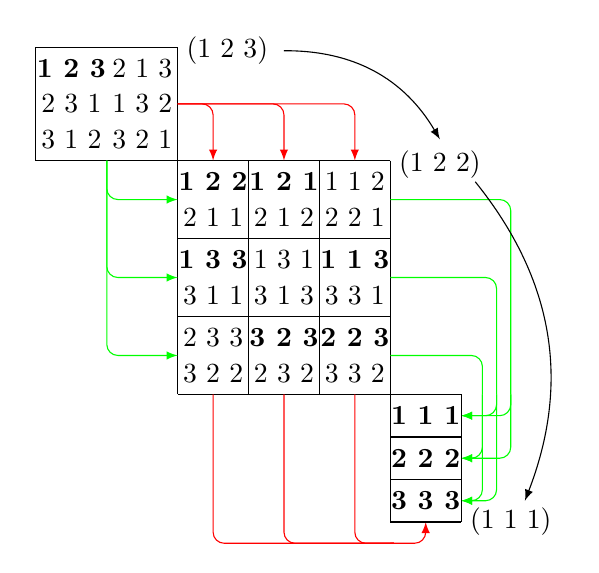
\begin{tikzpicture}[scale = 0.9]
	\tikzstyle{fleche}=[->,>=latex,rounded corners=4pt]
	\node at (2.2,0.25){$\jc$(1 2 3)};
	\node[font = \bfseries] at (0,0){1 2 3};
	\node at (0,-1/2){2 3 1};
	\node at (0,-1){3 1 2};
	\node at (1,0){2 1 3};
	\node at (1,-1/2){1 3 2};
	\node at (1,-1){3 2 1};
	
	
	\draw[black] (-.5,.3) to (1.5, .3);
	\draw[black] (-.5,.3) to (-.5, -1.3);
	\draw[black] (1.5,.3) to (1.5, -4.6);
	\draw[black] (-.5,-1.3) to (4.5, -1.3);
	
	\draw[fleche, red] (1.5,-1/2) -| (2, -1.3);
	\draw[fleche, red] (1.5,-1/2) -| (3, -1.3);
	\draw[fleche, red] (1.5,-1/2) -| (4, -1.3);
	\draw[fleche, green] (.5,-1.3) |- (1.5, -1.85);
	\draw[fleche, green] (.5,-1.3) |- (1.5, -2.95);
	\draw[fleche, green] (.5,-1.3) |- (1.5, -4.05);
	
	\node at (5.2,-1.6+0.25){$\jc$(1 2 2)};
	\draw[->,>=latex, bend left] (3,0.25) to (5.2,-1);
	\node[font = \bfseries] at (2,-1.6){1 2 2};
	\node at (2,-2.1){2 1 1};
	\node[font = \bfseries] at (3,-1.6){1 2 1};
	\node at (3,-2.1){2 1 2};
	\node at (4,-1.6){1 1 2};
	\node at (4,-2.1){2 2 1};
	
	\draw[black] (1.5, -2.4) to (4.5, -2.4);
	
	\node[font = \bfseries] at (2,-2.7){1 3 3};
	\node at (2,-3.2){3 1 1};
	\node at (3,-2.7){1 3 1};
	\node at (3,-3.2){3 1 3};
	\node[font = \bfseries] at (4,-2.7){1 1 3};
	\node at (4,-3.2){3 3 1};
	
	\draw[black] (1.5, -3.5) to (4.5, -3.5);
	
	\node at (2,-3.8){2 3 3};
	\node at (2,-4.3){3 2 2};
	\node[font = \bfseries] at (3,-3.8){3 2 3};
	\node at (3,-4.3){2 3 2};
	\node[font = \bfseries] at (4,-3.8){2 2 3};
	\node at (4,-4.3){3 3 2};
	
	\draw[black] (1.5, -4.6) to (5.5, -4.6);
	\draw[black] (2.5, -1.3) to (2.5, -4.6);
	\draw[black] (3.5, -1.3) to (3.5, -4.6);
	\draw[black] (4.5, -1.3) to (4.5, -6.4);
	
	\draw[rounded corners=4pt, red] (2, -4.6) |- (4.55, -6.7);
	\draw[rounded corners=4pt, red] (3, -4.6) |- (4.55, -6.7);
	\draw[rounded corners=4pt, red] (4, -4.6) |- (4.55, -6.7);
	\draw[fleche, red] (4.5, -6.7) -| (5, -6.4);
	\draw[rounded corners=4pt, green] (4.5, -1.85) -| (6.2, -4.6);
	\draw[fleche, green] (6.2, -4.6) |- (5.5, -4.9);
	\draw[fleche, green] (6.2, -4.6) |- (5.5, -5.5);
	\draw[rounded corners=4pt, green] (4.5, -2.95) -| (6, -4.6);
	\draw[fleche, green] (6, -4.6) |- (5.5, -4.9);
	\draw[fleche, green] (6, -4.6) |- (5.5, -6.1);
	\draw[rounded corners=4pt, green] (4.5, -4.05) -| (5.8, -4.6);
	\draw[fleche, green] (5.8, -4.6) |- (5.5, -6.1);
	\draw[fleche, green] (5.8, -4.6) |- (5.5, -5.5);
	
	\node at (6.2,-6.4){$\jc$(1 1 1)};
	\draw[->,>=latex, bend left] (5.7,-1.6) to (6.4,-6.1);
	\node[font = \bfseries] at (5, -4.9){1 1 1};
	\draw[black] (4.5, -5.2) to (5.5, -5.2);
	\node[font = \bfseries] at (5, -5.5){2 2 2};
	\draw[black] (4.5, -5.8) to (5.5, -5.8);
	\node[font = \bfseries] at (5, -6.1){3 3 3};
	
	\draw[black] (5.5, -4.6) to (5.5, -6.4);
	\draw[black] (4.5, -6.4) to (5.5, -6.4);
	
	\end{tikzpicture}
	\caption[Green relations in $T_3$.]{Green relations in $T_3$. \\ {\small Each block is a $\jc$-class, each line is a $\rc$-class, each column a $\lc$-class and each case an $\hc$-class. The red, green and black arrows represent the $\lc$, $\rc$ and $\jc$-order respectively.}}
\end{figure}\label{fig:green_t3}
			
	The following notations will prove useful, as the study of Green relations is, in part, the study of the maps given by left and right translations in the monoid.
	\begin{notation}\label{not:times}
		Let $h, k$ be elements of $M$ and $S$ be a subset of $M$. We denote by:
		\begin{itemize}
			\item $h\mul{S}$ the application from $S$ to $hS$ defined by $s \mapsto hs$,
			\item $\mul{S}k$ the application from $S$ to $Sk$ defined by $s \mapsto sk$,
			\item ${}_M\stab(S) = \{m \in M \sepp mS = S\}$,
			\item $\stab_M(S) = \{m \in M \sepp Sm = S\}$,
			\item $\fix_S(h, k) = \{s \in S \sepp hsk=s\}$.
		\end{itemize}
	\end{notation}
	
	Using these notations, let us recall Green's Lemma, which is one of the central elements of the theory of Green relations, as it shows that the structure of the relations is actually heavily constrained, making their study practical.
	
	\begin{lemme}[Green's Lemma]\label{lem:green}
		Let $a, a'$ be two elements in the same $\lc$-class and let $\lambda, \lambda'$ such that $\lambda a = a'$ and $\lambda' a' = a$. Then $\lambda\mul{\rc(a)}$ and $\lambda'\mul{\rc(a')}$ are reciprocal bijections. Moreover, for any $\lc$-class $L$ $\lambda\mul{\rc(a)\cap L}$ and $\lambda'\mul{\rc(a')\cap L}$ are reciprocal bijections.
		
		Similarly, if $a, b$ are two elements in the same $\rc$-class and $\rho, \rho'$ are such that $\rho a = b$ and $\rho' b = a$, then $\mul{\lc(a)}\rho$ and $\mul{\lc(b)}\rho'$ are reciprocal bijections. Moreover, for any $\rc$-class $R$ $\mul{\lc(a)\cap R}\rho$ and $\mul{\lc(b)\cap R}\rho'$ are reciprocal bijections.
	\end{lemme}
	
	\begin{figure}[h!]
	\centering
	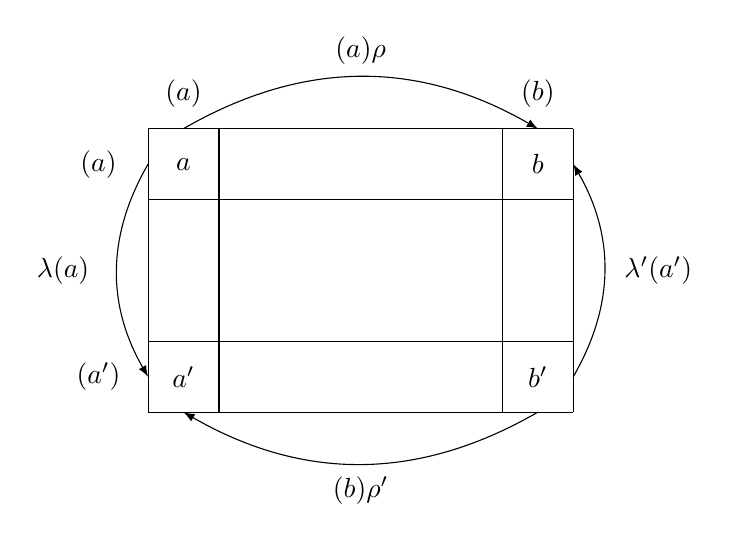
\begin{tikzpicture}[scale = 0.9]
	\tikzstyle{fleche}=[->,>=latex,rounded corners=4pt]
	\node at (0,0){$a'$};
	\node at (0,3){$a$};
	\node at (5,0){$b'$};
	\node at (5,3){$b$};
	\draw (-.5,3.5) -- (-.5, -.5);
	\draw (.5,3.5) -- (.5, -.5);
	\draw (5.5,3.5) -- (5.5, -.5);
	\draw (4.5,3.5) -- (4.5, -.5);
	\draw (-.5,3.5) -- (5.5, 3.5);
	\draw (-.5,2.5) -- (5.5, 2.5);
	\draw (-.5,.5) -- (5.5, .5);
	\draw (-.5,-.5) -- (5.5, -.5);
	
	\draw[->, >=latex, bend right] (-.5,3) to (-.5,0);
	\node at (-1.7, 1.5){$\lambda\mul{\rc(a)}$};
	\draw[->, >=latex, bend right] (5.5,0) to (5.5,3);
	\node at (6.7, 1.5){$\lambda'\mul{\rc(a')}$};
	\draw[->, >=latex, bend left] (0,3.5) to (5,3.5);
	\node at (2.5, 4.6){$\mul{\lc(a)}\rho$};
	\draw[->, >=latex, bend left] (5,-.5) to (0,-.5);
	\node at (2.5, -1.6){$\mul{\lc(b)}\rho'$};
	
	\node at (-1.2, 3){$\rc(a)$};
	\node at (-1.2, 0){$\rc(a')$};
	\node at (0, 4){$\lc(a)$};
	\node at (5, 4){$\lc(b)$};
	
	\end{tikzpicture}
	\caption{Green's Lemma}
\end{figure}
	
	An important consequence of Green's Lemma is that $\jc$-classes can be neatly organized as \emph{eggbox pictures}\footnote{Terminology introduced in \cite{clifford1961algebraic}}: the $\jc$-class can be represented as a rectangular array with the $\lc$-classes as columns, the $\rc$-classes as rows and the $\hc$-classes, the eggs, in the cases, as can be seen in Figure \ref{fig:green_t3}. This level organization is actually what allows for efficient computer representation of monoids and most of their algorithmic exploration. 
	
	\subsubsection{\schu groups}
	
	The Green structure offers a second way of facilitating computer exploration of monoids through groups that arise as stabilizers of some Green classes. These are called the \emph{\schu groups} and -- this a running theme of monoid theory -- allow for a number of monoid theoretic questions to be formulated in terms of groups for which we dispose of an array of efficient algorithms.
	
	\begin{dftn}[\schu groups]\label{def:schu_groups}
		Let $H$ be an $\hc$-class. The set $\{ h\mul{H} \sepp h \in {}_M\stab(H)\}$ equipped with map composition is a subgroup of $\symm(H)$ called the \emph{left \schu group} and denoted by $\Gamma(H)$.
		
		Similarly, $(\{ \mul{H}k \sepp k \in \stab_M(H)\}, \circ)$ is a subgroup of $\symm(H)$ called the \emph{right \schu group} and denoted by $\Gamma'(H)$.
	\end{dftn}

	\begin{lined}
		\begin{ex}\label{ex:schu_as_symm}
			Consider $H = \hc([1\ 3\ 1])$ (the elements of $T_n$ are given in function notation in all examples). We have :
			\[{}_M\stab(H) = \{[1\ 2\ 3], [3\ 2\ 1], [1\ 3\ 3], [3\ 1\ 1], [1\ 1\ 3], [3\ 3\ 1]\}\]
			and subsequently, $\Gamma(H) = \{[1\ 2\ 3]\mul{H}, [3\ 3\ 1]\mul{H}\}$. Notice that, as elements of $\Gamma(H)$, $[3\ 3\ 1]\mul{H} = [3\ 2\ 1]\mul{H}$ and that the only important thing is the permutations induced by the elements of ${}_M\stab(H)$ on $\im H$. Thus, in the case of transformation monoids, the left \schu group of an $\hc$-class $H$ can be represented as a subgroup of $\symm(\im H)$. In the same way, the right \schu groups can be represented as subgroups of $\symm(\ker H)$. This fact is used to represent the \schu groups in Section \ref{sec:Algos}.
		\end{ex}
	\end{lined}

	Our precedent remark on exploiting \schu groups to get efficient algorithms for computational monoid theoretic questions is seconded by the fact that \schu groups do not contain any "superfluous information" in the following sense.
	
	\begin{prop}\label{prop:schu_acts_freely}
		Let $H$ be an $\hc$-class. The natural actions of  $\Gamma(H)$ and $\Gamma'(H)$ on $H$ are free and transitive.
	\end{prop}
	
	We reproduce below a proof for Proposition \ref{prop:schu_acts_freely} from \cite{schu} for the purpose of showcasing the main argument. The argument itself is widely known and we will use it multiple times in the remainder of this paper.
	
	\begin{proof}
		 Two elements $h, h' \in H$ are in the same $\lc$-class so there is some $u \in M$ such that $uh=h'$. By Green's Lemma, this means that $u \in {}_M\stab(H)$, so $\Gamma(H)$ acts transitively on $H$. Suppose that $uh = h$ for some $u\in M$. Since $h, h'$ are also in the same $\rc$ class, there is some $v$ such that $h' = hv$, so $uh'=uhv=hv=h'$ : an element of $\Gamma(H)$ either fixes all points in $H$ or fixes none. The only element of $\Gamma(H)$ that fixes all points (and, consequently, the only one that fixes any point) is the identity and thus the action is free. The same arguments apply for $\Gamma'(H)$.
	\end{proof}
	
	A special case that is interesting to note, and that will be important later, it the case where $H$ is the $\hc$-class of an idempotent :
	
	\begin{dftn}\label{dftn:idem_and_maxgrp}
		An element $e \in M$ is \emph{idempotent} if $e^2=e$. Given an idempotent $e$, the set $G_e = \{x \in M\sepp \exists y \in M, xy=yx=e\}$ is called the \emph{maximal subgroup at $e$}. One can check that $G_e$ is indeed a group and that $G_e = \hc(e)$.
	\end{dftn}

	In that case, $\Gamma(H)$ and $\Gamma'(H)$ can be defined as before, and are canonically isomorphic to $G_e$, simply because $G_e \subset {}_M\stab(H)$ naturally induce a map making it a subgroup of $\Gamma(H)$ and that since $G_e$ acts freely and transitively on $H$, this map must be injective and surjective (and similarly for $\Gamma'(H)$).
	
	\begin{lined}
		\begin{ex}\label{ex:iso_idem}
			Consider, in Example \ref{ex:green_tn}, $e = [1\ 2\ 2]$ and $H = \hc(e)$. $e$ is an idempotent, and, indeed, $H = G_e$ is group : setting $t = [2\ 1\ 1]$, we have $e^2=e, t^2=e$ and $et=te=t$.
			As noted in Example \ref{ex:schu_as_symm} :
			\[\Gamma(H) = \symm(\{1, 2\}), \qquad \Gamma'(H) = \symm(\{\{1\}, \{2,3\}\}).\]
			Note that the canonical isomorphism between $\Gamma(H)$ and $\hc(e)$ is simply given by $g \in \Gamma(H) \mapsto g \cdot e \in H$.
		\end{ex}
	\end{lined}